%==============================================================
%  EE201 -- Circuit Theory I
%  Lecture 5 : The Inductor
%  M. Mert Ankaralı, METU EEE
%
%  Compile:  ./build.sh      (or: pdflatex EE201_Lecture_5.tex, twice)
%==============================================================
\documentclass[11pt,a4paper]{article}

%-------------------- packages --------------------------------
\usepackage[T1]{fontenc}
\usepackage[utf8]{inputenc}
\usepackage[english]{babel}
\usepackage{lmodern}
\usepackage[margin=2.3cm,top=2.0cm,bottom=1.9cm,headheight=14pt,headsep=9pt]{geometry}
\usepackage{amsmath,amssymb}
\usepackage{array,booktabs,tabularx}
\usepackage{enumitem}
\usepackage[table]{xcolor}
\usepackage{fancyhdr}
\usepackage{titlesec}
\usepackage{graphicx}
\usepackage[most]{tcolorbox}
\usepackage{tikz}
\usepackage[american,siunitx]{circuitikz}
\usetikzlibrary{arrows.meta,positioning,calc,decorations.pathmorphing,decorations.pathreplacing,decorations.markings,patterns,shapes.geometric}
\usepackage[colorlinks=true,allcolors=metured,breaklinks=true]{hyperref}

%-------------------- colour system ---------------------------
% One colour per physical quantity, used identically in the slides.
\definecolor{metured}{RGB}{155,27,48}    % headings, structure
\definecolor{metugray}{RGB}{88,89,91}
\definecolor{ccur}{RGB}{0,102,170}       % CURRENT  -- blue
\definecolor{cvolt}{RGB}{214,120,0}      % VOLTAGE  -- orange
\definecolor{cpow}{RGB}{23,128,74}       % POWER / ENERGY -- green
\definecolor{ccharge}{RGB}{124,60,160}   % CHARGE   -- purple
\definecolor{cflux}{RGB}{0,138,138}      % FLUX LINKAGE -- teal
\definecolor{boxgray}{RGB}{245,245,245}

\newcommand{\Icol}[1]{\textcolor{ccur}{#1}}
\newcommand{\Vcol}[1]{\textcolor{cvolt}{#1}}
\newcommand{\Pcol}[1]{\textcolor{cpow}{#1}}
\newcommand{\Qcol}[1]{\textcolor{ccharge}{#1}}
\newcommand{\Fcol}[1]{\textcolor{cflux}{#1}}

%-------------------- units (no siunitx dependency) -----------
\newcommand{\uni}[1]{\,\mathrm{#1}}
\newcommand{\A}{\uni{A}}   \newcommand{\V}{\uni{V}}
\newcommand{\W}{\uni{W}}   \newcommand{\J}{\uni{J}}
\newcommand{\Cb}{\uni{C}}  \newcommand{\s}{\uni{s}}
\newcommand{\Wb}{\uni{Wb}}  \newcommand{\Hy}{\uni{H}}

%-------------------- layout ----------------------------------
\pagestyle{fancy}
\fancyhf{}
\lhead{\small\textcolor{metugray}{EE201 -- Circuit Theory I}}
\rhead{\small\textcolor{metugray}{Lecture 5: The Inductor}}
\cfoot{\small\thepage}
\renewcommand{\headrulewidth}{0.4pt}

\titleformat{\section}{\large\bfseries\color{metured}}{\thesection.}{0.6em}{}
\titleformat{\subsection}{\normalsize\bfseries\color{metugray}}{\thesubsection.}{0.6em}{}
\titlespacing*{\section}{0pt}{1.4ex plus .3ex}{0.7ex}
\titlespacing*{\subsection}{0pt}{1.1ex plus .2ex}{0.5ex}

\setlist[itemize]{itemsep=2pt,topsep=3pt,parsep=0pt,leftmargin=1.5em}
\setlist[enumerate]{itemsep=2pt,topsep=3pt,parsep=0pt,leftmargin=1.7em}
\setlength{\parindent}{0pt}
\setlength{\parskip}{0.7ex plus .1ex}
\raggedbottom
\widowpenalty=10000
\clubpenalty=10000
\brokenpenalty=10000

%-------------------- boxes -----------------------------------
\newtcolorbox{definitionbox}[1]{enhanced,
  colback=metured!4, colframe=metured, boxrule=0.9pt,
  fonttitle=\bfseries, title={#1}, arc=2pt,
  left=7pt,right=7pt,top=5pt,bottom=5pt, before skip=7pt, after skip=7pt}

\newtcolorbox{ideabox}[1][Key idea]{enhanced,
  colback=ccur!5, colframe=ccur, boxrule=0.9pt,
  fonttitle=\bfseries, title={#1}, arc=2pt,
  left=7pt,right=7pt,top=5pt,bottom=5pt, before skip=7pt, after skip=7pt}

\newtcolorbox{examplebox}[1][Example]{enhanced,
  colback=cpow!4, colframe=cpow, boxrule=0.9pt,
  fonttitle=\bfseries, title={#1}, arc=2pt,
  left=7pt,right=7pt,top=5pt,bottom=5pt, before skip=7pt, after skip=7pt}

\newtcolorbox{cautionbox}[1][Careful]{enhanced,
  colback=cvolt!6, colframe=cvolt, boxrule=0.9pt,
  fonttitle=\bfseries, title={#1}, arc=2pt,
  left=7pt,right=7pt,top=5pt,bottom=5pt, before skip=7pt, after skip=7pt}

%-------------------- circuitikz defaults ---------------------
\ctikzset{bipoles/length=0.9cm, color=black,
          label/align=straight,
          bipoles/vsourceam/height=0.85, bipoles/vsourceam/width=0.85}
\tikzset{
  curarr/.style={-{Stealth[length=2.6mm]}, ccur, very thick},
  volarr/.style={-{Stealth[length=2.6mm]}, cvolt, very thick},
  blk/.style={draw=metugray, fill=boxgray, rounded corners=2pt,
              minimum height=1.25cm, text width=2.9cm, align=center, font=\small},
  flowarr/.style={-{Stealth[length=3mm]}, metured, very thick},
}

%==============================================================

%-------------------- extra macros for this lecture -----------
\newcommand{\ohm}{\,\Omega}
\newcommand{\kohm}{\,\mathrm{k}\Omega}
\newcommand{\Req}{R_{\mathrm{eq}}}
%  v--i axes:  #1 half-width, #2 half-height, #3 caption under the frame
\newcommand{\viaxes}[3]{%
  \draw[vax] (-#1,0) -- (#1,0) node[right=1pt, font=\scriptsize, text=cvolt] {$v$};
  \draw[vax] (0,-#2) -- (0,#2) node[above=1pt, font=\scriptsize, text=ccur] {$i$};
  \node[ttl] at (0,-#2-0.68) {#3};}
%  q--v axes: voltage across, charge stored
\newcommand{\qvaxes}[3]{%
  \draw[vax] (-#1,0) -- (#1,0) node[right=1pt, font=\scriptsize, text=cvolt] {$v$};
  \draw[vax] (0,-#2) -- (0,#2) node[above=1pt, font=\scriptsize, text=ccharge] {$q$};
  \node[ttl] at (0,-#2-0.68) {#3};}
%  i--phi axes: current through, flux linkage stored
\newcommand{\iphiaxes}[3]{%
  \draw[vax] (-#1,0) -- (#1,0) node[right=1pt, font=\scriptsize, text=ccur] {$i$};
  \draw[vax] (0,-#2) -- (0,#2) node[above=1pt, font=\scriptsize, text=cflux] {$\varphi$};
  \node[ttl] at (0,-#2-0.68) {#3};}
%  t axes for waveforms
\newcommand{\taxes}[4]{%
  \draw[vax] (-0.15,0) -- (#1,0) node[right=1pt, font=\scriptsize] {$t$};
  \draw[vax] (0,-#2) -- (0,#3) node[above=1pt, font=\scriptsize] {#4};}
\tikzset{
  gnode/.style={circle, fill=metured, inner sep=0pt, minimum size=4.2pt},
  glab/.style={font=\footnotesize, text=metured},
  barr/.style={-{Stealth[length=2.2mm]}, metugray, thick},
  surf/.style={draw=cpow, very thick, dashed, rounded corners=6pt},
  vax/.style={-{Stealth[length=2mm]}, gray!70},
  crv/.style={metured, very thick},
  ttl/.style={font=\scriptsize\bfseries, text=metugray},
  gbr/.style={metugray, thick, postaction={decorate, decoration={markings,
      mark=at position 0.58 with {\arrow{Stealth[length=2.4mm]}}}}},
  pol/.style={font=\small, text=cvolt},
  iar/.style={-{Stealth[length=2.4mm]}, ccur, very thick},
}

%==============================================================
\begin{document}

%-------------------- title block -----------------------------
\begin{center}
\begin{tcolorbox}[enhanced, colback=metured!5, colframe=metured, boxrule=1pt,
                  arc=3pt, left=10pt,right=10pt,top=7pt,bottom=7pt, width=\textwidth]
\begin{center}
  {\small\scshape Middle East Technical University}\\[2pt]
  {\small\scshape Department of Electrical and Electronics Engineering}\\[7pt]
  {\Large\bfseries\color{metured} EE201 -- Circuit Theory I}\\[4pt]
  {\large\bfseries Lecture 5: The Inductor\\ and a summary of the LTI elements}\\[6pt]
  {\small M. Mert Ankaralı}
\end{center}
\end{tcolorbox}
\end{center}
\vspace{-0.5em}

\begin{center}
\small
\begin{tabular}{@{}l l@{}}
\toprule
\multicolumn{2}{@{}l}{\textbf{Colour code used in these notes and in the slides}}\\
\midrule
\Fcol{$\blacksquare$}~flux linkage $\varphi$ & \Icol{$\blacksquare$}~current $i$ \quad
\Vcol{$\blacksquare$}~voltage $v$ \quad \Qcol{$\blacksquare$}~charge $q$ \quad
\Pcol{$\blacksquare$}~power $p$, energy $w$\\
\bottomrule
\end{tabular}
\end{center}

%==============================================================
\section{The other way to store energy}

Lecture~4 gave us an element that dissipates nothing: the capacitor holds energy in the
electric field between its plates and hands it back when asked. Today's element does the
same job with the other field --- drive a current through a coil of wire and the magnetic
field that appears holds energy too.

\begin{center}
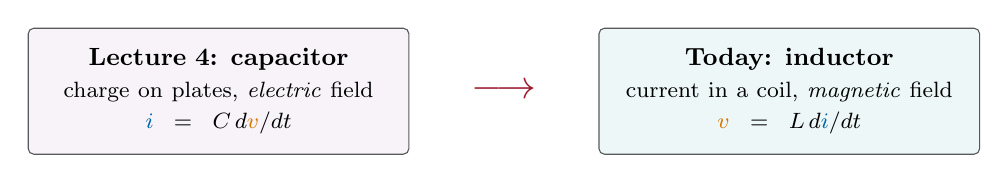
\begin{tikzpicture}[node distance=0.9cm]
  \node[blk, text width=4.6cm, minimum height=1.6cm, fill=ccharge!6] (a)
       {\textbf{Lecture 4: capacitor}\\[2pt]\footnotesize charge on plates,
        \emph{electric} field\\ \footnotesize $\Icol{i} = C\,d\Vcol{v}/dt$};
  \node[blk, text width=4.6cm, minimum height=1.6cm, right=2.4cm of a, fill=cflux!7] (b)
       {\textbf{Today: inductor}\\[2pt]\footnotesize current in a coil,
        \emph{magnetic} field\\ \footnotesize $\Vcol{v} = L\,d\Icol{i}/dt$};
  \node[font=\Large, text=metured] at ($(a)!0.5!(b)$) {$\longrightarrow$};
\end{tikzpicture}
\end{center}

The two terminal equations above are the same equation with $\Vcol{v}$ and $\Icol{i}$
exchanged. That is no coincidence: almost everything proved about the capacitor becomes
true of the inductor once you swap voltage for current. We will still build it from the
ground up --- but try to guess each result before it appears.

%==============================================================
\section{The coil, and the voltage it pushes back with}

Start from something you can watch on a bench without knowing any field theory. Wind a
length of wire into a coil and drive a current through it.

Two words: the \textbf{coil} is the object you just wound; the \textbf{inductor} is the
circuit element we model it with, and that is the word we use from here on. (A real coil
is an inductor plus the resistance of its own wire.)

\begin{center}
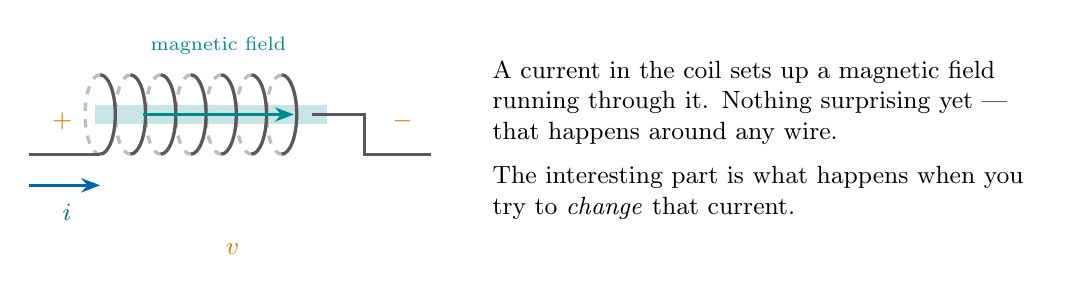
\begin{tikzpicture}[x=1.2cm,y=1.2cm]
\draw[cflux!22, line width=7pt] (0.0,0.97) -- (2.45,0.97);
\draw[metugray, very thick] (-0.7,0.55) -- (0.05,0.55);
\foreach \k in {0,...,6}{
  \draw[metugray, very thick] (0.05+0.32*\k,0.55) arc (-90:90:0.16 and 0.42);
  \draw[metugray, very thick, dashed, opacity=0.40]
        (0.05+0.32*\k,1.39) arc (90:270:0.16 and 0.42);}
\draw[metugray, very thick] (2.29,0.97) -- (2.85,0.97) -- (2.85,0.55) -- (3.55,0.55);
\draw[iar] (-0.7,0.22) -- (0.05,0.22); \node[ccur, font=\small] at (-0.3,-0.06) {$i$};
\draw[cflux, very thick, -{Stealth[length=2.4mm]}] (0.5,0.97) -- (2.1,0.97);
\node[font=\scriptsize, text=cflux] at (1.3,1.70) {magnetic field};
\node[pol] at (-0.35,0.90) {$+$};  \node[pol] at (3.25,0.90) {$-$};
\node[pol] at (1.45,-0.45) {$\Vcol{v}$};
\node[font=\small, anchor=west, text width=6.8cm] at (4.1,0.7)
  {A current in the coil sets up a magnetic field running through it. Nothing surprising
   yet --- that happens around any wire.\\[5pt]
   The interesting part is what happens when you try to \emph{change} that current.};
\end{tikzpicture}
\end{center}
\vspace{4pt}

Push the current up and the inductor develops a voltage that \emph{opposes} you; let it
fall and that voltage reverses, now trying to keep the current going. The faster the
change, the larger the voltage.

\begin{center}
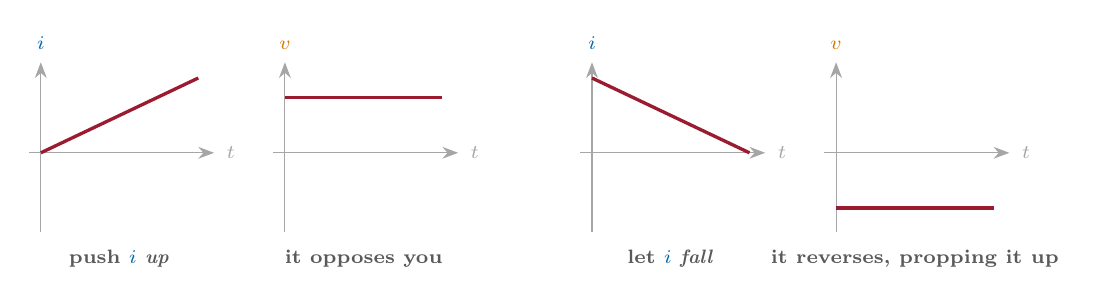
\begin{tikzpicture}[x=1cm,y=1cm]
\begin{scope}
  \taxes{2.2}{1.0}{1.15}{\Icol{$i$}}
  \draw[crv] (0,0) -- (2.0,0.95);
  \node[ttl] at (1.0,-1.35) {push $\Icol{i}$ \emph{up}};
\end{scope}
\begin{scope}[xshift=3.1cm]
  \taxes{2.2}{1.0}{1.15}{\Vcol{$v$}}
  \draw[crv] (0,0.7) -- (2.0,0.7);
  \node[ttl] at (1.0,-1.35) {it opposes you};
\end{scope}
\begin{scope}[xshift=7.0cm]
  \taxes{2.2}{1.0}{1.15}{\Icol{$i$}}
  \draw[crv] (0,0.95) -- (2.0,0);
  \node[ttl] at (1.0,-1.35) {let $\Icol{i}$ \emph{fall}};
\end{scope}
\begin{scope}[xshift=10.1cm]
  \taxes{2.2}{1.0}{1.15}{\Vcol{$v$}}
  \draw[crv] (0,-0.7) -- (2.0,-0.7);
  \node[ttl] at (1.0,-1.35) {it reverses, propping it up};
\end{scope}
\end{tikzpicture}
\end{center}
\vspace{2pt}

\begin{definitionbox}{Back EMF}
The voltage an inductor develops when its current changes is called the \textbf{back EMF}
(``electromotive force'' is a historical name --- it is a voltage). It always acts so as to
\emph{oppose the change} that produced it: it fights a rising current and props up a
falling one.\\[4pt]
Keep the \textbf{passive sign convention} and the marks never move: with $\Icol{i}$
referenced into the $+$ terminal, a rising current simply makes $\Vcol{v}$ positive and a
falling one makes it negative. The opposition shows up in the \emph{sign} of $\Vcol{v}$,
never in a redrawn polarity.
\end{definitionbox}

\section{Inductance: how hard it pushes back}

Two inductors in the same circuit will not push back equally. The constant of proportionality
in $\Vcol{v} \propto d\Icol{i}/dt$ is the \textbf{inductance} $L$:
\[
  \boxed{\;\Vcol{v} \;=\; L\,\frac{d\Icol{i}}{dt}\;}
  \qquad\qquad
  1\Hy \;=\; 1\,\frac{\mathrm{V}\cdot\mathrm{s}}{\mathrm{A}} .
\]
Read the unit as the definition: one henry is the inductance that produces one volt of
back EMF when the current is rising at one ampere per second.

\begin{ideabox}[$L$ grows with]
\begin{itemize}
  \item the \textbf{number of turns} --- each extra turn catches the field again, so $L$
        grows faster than the turn count itself;
  \item the \textbf{shape}: long and thin, or short and fat, differs even for the same
        wire;
  \item and above all \textbf{what is inside it} --- an iron core instead of air
        multiplies $L$ by hundreds.
\end{itemize}
\end{ideabox}
\vspace{2pt}

\begin{cautionbox}[One henry is large]
A 1000-turn coil, $1\uni{cm}^2$ in section and $5\uni{cm}$ long, wound on air, comes to
about $2.5\uni{mH}$. Practical values run from nH to a few mH; reaching henries means an
iron core. Compare Lecture~4: one farad was enormous for exactly the same reason.
\end{cautionbox}

\section{Volt-seconds: the inductor's version of charge}

We have the terminal equation, but not yet the \emph{characteristic} --- the curve that
says what kind of element this is. Lecture~4 found the capacitor's by asking what was being
accumulated: $\Qcol{q} = \int \Icol{i}\,d\tau$, in \emph{amp-seconds}, which we call
coulombs. The inductor asks the same of the other variable. Integrate the voltage:

\begin{definitionbox}{Flux linkage}
\vspace{-8pt}
\[
  \Fcol{\varphi(t)} \;=\; \Fcol{\varphi(t_0)} + \int_{t_0}^{t}\!\Vcol{v(\tau)}\,d\tau
  \qquad\Longleftrightarrow\qquad
  \Vcol{v} \;=\; \frac{d\Fcol{\varphi}}{dt}
\]
\vspace{-14pt}
\end{definitionbox}

That integral is measured in \emph{volt-seconds}, and a volt-second has a name of its own:
the \textbf{weber} (Wb).

\begin{center}
\small
\renewcommand{\arraystretch}{1.15}
\begin{tabular}{@{}l l l@{}}
\toprule
 & \textbf{capacitor} \footnotesize(Lecture 4) & \textbf{inductor} \footnotesize(today)\\
\midrule
accumulate which variable? & the current $\Icol{i}$ & the voltage $\Vcol{v}$\\
the running total & $\Qcol{q} = \int\!\Icol{i}\,d\tau$ & $\Fcol{\varphi} = \int\!\Vcol{v}\,d\tau$\\
measured in & amp-seconds $=$ coulombs & volt-seconds $=$ webers\\
so & $\Icol{i} = d\Qcol{q}/dt$ & $\Vcol{v} = d\Fcol{\varphi}/dt$\\
\bottomrule
\end{tabular}
\end{center}
\vspace{4pt}

\subsection{Why it is called \emph{flux linkage}}

Because $\Fcol{\varphi}$ is the magnetic field inside the winding, counted once for every
turn it passes through. More turns, a fatter winding, or iron instead of air all mean more
field and so a larger $\Fcol{\varphi}$ --- the same three things that made $L$ large. And
a \emph{changing} $\Fcol{\varphi}$ is the back EMF, which is Faraday's law.

One difference from Lecture~4 is worth naming. Charge is countable stuff --- so many
coulombs of electrons on a plate. Volt-seconds are not a substance and nothing is piling
up anywhere; $\Fcol{\varphi}$ is a bookkeeping variable. But it behaves, in every equation
from here on, exactly as charge did.

\begin{definitionbox}{Inductor}
A two-terminal element is an \textbf{inductor} if, at every instant, its
$(\Icol{i},\Fcol{\varphi})$ pairs lie on a curve in the $\Icol{i}$--$\Fcol{\varphi}$ plane.
\end{definitionbox}

\begin{center}
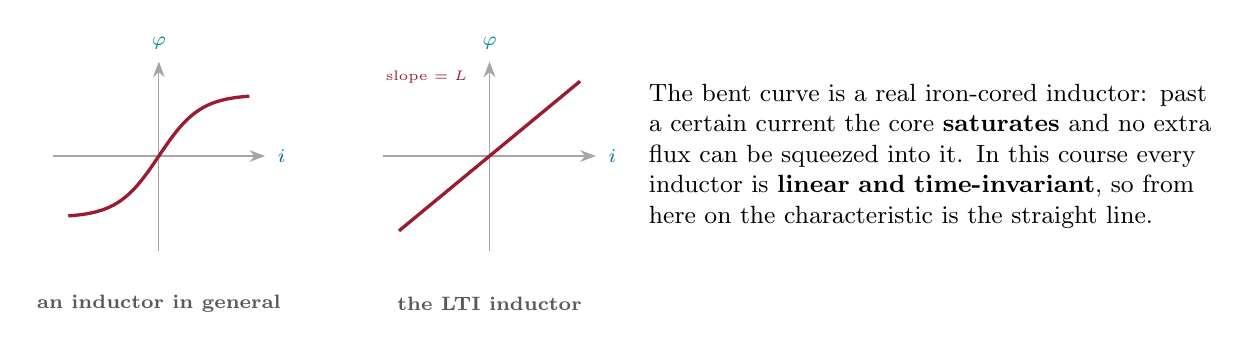
\begin{tikzpicture}[x=1cm,y=1cm]
\begin{scope}
  \iphiaxes{1.35}{1.2}{an inductor in general}
  \draw[crv, domain=-1.15:1.15, samples=140, smooth] plot (\x, {0.78*tanh(1.9*\x)});
\end{scope}
\begin{scope}[xshift=4.2cm]
  \iphiaxes{1.35}{1.2}{the LTI inductor}
  \draw[crv] (-1.15,-0.95) -- (1.15,0.95);
  \node[font=\tiny, text=metured] at (-0.80,1.00) {slope $=L$};
\end{scope}
\node[font=\small, anchor=west, text width=7.2cm] at (6.1,0)
  {The bent curve is a real iron-cored inductor: past a certain current the core
   \textbf{saturates} and no extra flux can be squeezed into it. In this course every
   inductor is \textbf{linear and time-invariant}, so from here on the characteristic is
   the straight line.};
\end{tikzpicture}
\end{center}
\vspace{2pt}

And again, note what has \emph{not} happened. There is no relation between the values of
$\Vcol{v}$ and $\Icol{i}$ at one instant: no function $f$ or $g$ with
\[
  \Vcol{v(t)} = f\bigl(\Icol{i(t)}\bigr)
  \qquad\text{or}\qquad
  \Icol{i(t)} = g\bigl(\Vcol{v(t)}\bigr) .
\]
Fix the current and the voltage is still free --- it depends on how $\Icol{i}$ is
\emph{changing}, not on what it is. An inductor is not a resistor either, and it has no
characteristic in the $\Vcol{v}$--$\Icol{i}$ plane.

\section{The LTI inductor}
\label{sec:lti}

\begin{definitionbox}{LTI inductor}
The $\Icol{i}$--$\Fcol{\varphi}$ characteristic is a fixed straight line through the
origin, $\Fcol{\varphi} = L\,\Icol{i}$ --- and its slope is the same $L$ we met in
Section~3. Differentiating and using $\Vcol{v} = d\Fcol{\varphi}/dt$ gives back the
terminal equation, now with a characteristic behind it:
\[
  \boxed{\;\Vcol{v} \;=\; L\,\frac{d\Icol{i}}{dt}\;}
  \qquad\text{or, integrated,}\qquad
  \boxed{\;\Icol{i(t)} = \Icol{i(t_0)} + \frac{1}{L}\int_{t_0}^{t}\!\Vcol{v(\tau)}\,d\tau\;}
\]
\end{definitionbox}

\begin{center}
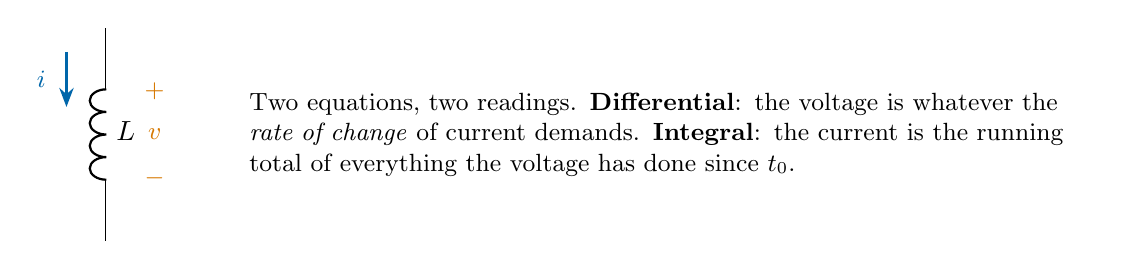
\begin{tikzpicture}[scale=1.0]
  \draw (0,-0.35) -- (0,0) to[L, l_=$L$] (0,2.0) -- (0,2.35);
  \node[pol] at (0.62,1.55) {$+$}; \node[pol] at (0.62,0.45) {$-$};
  \node[pol] at (0.62,1.0) {$v$};
  \draw[iar] (-0.5,2.05) -- (-0.5,1.35);
  \node[ccur, font=\small] at (-0.82,1.7) {$i$};
  \node[font=\small, anchor=west, text width=10.6cm] at (1.7,1.0)
    {Two equations, two readings. \textbf{Differential}: the voltage is whatever the
     \emph{rate of change} of current demands. \textbf{Integral}: the current is the
     running total of everything the voltage has done since $t_0$.};
\end{tikzpicture}
\end{center}
\vspace{2pt}

\begin{ideabox}[Four things that follow --- each one the capacitor's, mirrored]
\begin{itemize}
  \item \textbf{At DC it is a short circuit.} $\Icol{i}$ constant $\Rightarrow
        d\Icol{i}/dt = 0 \Rightarrow \Vcol{v} = 0$, whatever the current is. To a DC
        source, an inductor is just a piece of wire.
  \item \textbf{Its current is continuous.} Flip a switch, step the source: the
        inductor's current is the \emph{same} an instant after as an instant before.
        Changing it takes time, because a jump would need an infinite voltage.
  \item \textbf{It remembers.} $\Icol{i(t)}$ depends on the whole history of $\Vcol{v}$,
        not on its present value.
  \item \textbf{It holds energy}, and the amount is $\Pcol{w} = \tfrac12 L\Icol{i}^{\,2}$
        --- fixed by the present current alone. Section~\ref{sec:energy} shows why, and
        that all of it can be taken back out.
\end{itemize}
\end{ideabox}

%==============================================================

%==============================================================
\begin{examplebox}[Example 5.1 --- a constant voltage across an inductor]
Hold $\Vcol{v} = 5\V$ across $L = 10\uni{mH}$, starting from $\Icol{i(0)} = 0$. The
integral form gives
\[
  \Icol{i(t)} = \frac{1}{L}\int_0^t 5\,d\tau = \frac{5}{10^{-2}}\,t = 500\,t \ \ [\mathrm{A}] .
\]
A \textbf{ramp}: the current climbs at $500\uni{A/s}$, reaching $5\A$ after $10\uni{ms}$.
Nothing about $\Icol{i}$ can be read off $\Vcol{v}$ at one instant --- only from the area
under it. This is Example~4.1 with the variables swapped, and it is why a real inductor
across a battery ends up limited by the resistance of its own wire.
\end{examplebox}

\begin{examplebox}[Example 5.2 --- opening a switch, and where the spark comes from]
An inductor carries a steady current $I_0$. Now open a switch in series with it: the
current is forced to $0$ in zero time.

\begin{center}
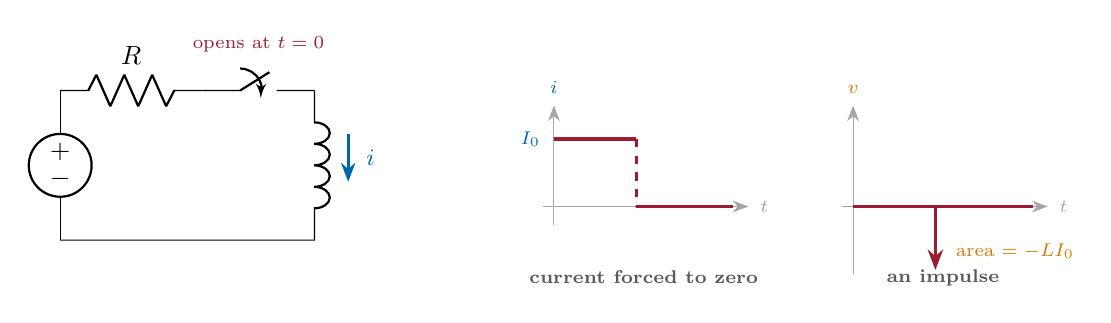
\begin{tikzpicture}[scale=0.95, transform shape]
\begin{scope}
  \draw (0,0) to[american voltage source, invert] (0,2.0);
  \draw (0,2.0) to[R, l=$R$] (1.9,2.0);
  \draw (1.9,2.0) to[cspst] (3.4,2.0);
  \node[font=\scriptsize, text=metured] at (2.65,2.62) {opens at $t=0$};
  \draw (3.4,2.0) to[L] (3.4,0) -- (0,0);
  \draw[iar] (3.85,1.42) -- (3.85,0.78);
  \node[ccur, font=\small] at (4.15,1.1) {$i$};
\end{scope}
\begin{scope}[xshift=6.6cm, yshift=0.45cm]
  \taxes{2.6}{0.25}{1.35}{\Icol{$i$}}
  \draw[crv] (0,0.9) -- (1.1,0.9);
  \draw[crv, dashed] (1.1,0.9) -- (1.1,0);
  \draw[crv] (1.1,0) -- (2.4,0);
  \node[font=\scriptsize, text=ccur, left] at (-0.06,0.9) {$I_0$};
  \node[ttl] at (1.2,-0.95) {current forced to zero};
\end{scope}
\begin{scope}[xshift=10.6cm, yshift=0.45cm]
  \taxes{2.6}{0.9}{1.35}{\Vcol{$v$}}
  \draw[crv] (0,0) -- (1.1,0);
  \draw[crv, -{Stealth[length=2.6mm]}] (1.1,0) -- (1.1,-0.85);
  \draw[crv] (1.1,0) -- (2.4,0);
  \node[font=\scriptsize, text=cvolt, right=2pt] at (1.18,-0.6) {area $= -LI_0$};
  \node[ttl] at (1.2,-0.95) {an impulse};
\end{scope}
\end{tikzpicture}
\end{center}
\vspace{-2pt}

A step of $-I_0$ in the current means $d\Icol{i}/dt = -I_0\,\delta(t)$, so
\[
  \Vcol{v(t)} \;=\; L\,\frac{d\Icol{i}}{dt} \;=\; -L I_0\,\delta(t) ,
\]
an impulse of area $-LI_0$. This is the exact mirror of Example~4.2, where an ideal
voltage step across a capacitor demanded a current impulse --- and it is just as much an
idealisation too far. What really happens is that the voltage across the opening contacts
climbs until the air between them breaks down, and the stored $\tfrac12 LI_0^2$ leaves as
a spark. The effect is a nuisance in switches and relays, and the whole point of an
ignition coil.
\end{examplebox}

%==============================================================
\section{Power and energy in an LTI inductor}
\label{sec:energy}

Follow the current up from zero and the stored energy falls out on its own.

At $t = 0$ the current is zero. To get current flowing you have to raise it --- and the
moment you do, the inductor answers with its back EMF $\Vcol{v} = L\,d\Icol{i}/dt$,
pointing \emph{against} you. So whatever is driving the circuit is pushing current through
an element that is pushing back, which means it is doing work, at a rate
$\Pcol{p} = \Vcol{v}\,\Icol{i} = L\,\Icol{i}\,d\Icol{i}/dt$. Add that up from
$\Icol{i} = 0$ to $\Icol{i} = I$, changing the variable of integration from $t$ to
$\Icol{i}$:
\[
  \int_0^{t}\! L\,\Icol{i}\,\frac{d\Icol{i}}{d\tau}\,d\tau
  \;=\; \int_0^{I}\! L\,\Icol{i}\,d\Icol{i}
  \qquad\Longrightarrow\qquad
  \boxed{\;\Pcol{w} \;=\; \tfrac12 L\,\Icol{i}^{\,2}
    \;=\; \frac{\Fcol{\varphi}^{\,2}}{2L}\;}
\]
No resistance was involved, so none of that work turned into heat: it is still there, and
the amount depends only on the present current. Differentiated, the same statement reads
$\Pcol{p} = \frac{d}{dt}(\tfrac12 L\Icol{i}^{\,2})$ --- power is the rate of change of the
stored energy.

Now run it backwards. Let the current fall: $d\Icol{i}/dt < 0$, so $\Vcol{v}$ changes sign,
and the inductor stops resisting the current and starts \emph{driving} it. $\Pcol{p}$ is
negative, and the element hands back exactly what it was given. Example~5.2 is that
handover done violently --- all of it at once, into a spark.

$\Pcol{w} \ge 0$ always, so an inductor can never give out more than it has been given: it
is \textbf{passive}. And nothing is lost on the way in or on the way out:
\textbf{lossless}.

\begin{ideabox}[So where was the energy kept?]
In the \textbf{magnetic field} the current set up inside the winding --- not in the wire, and
not in the moving charge itself. That is the only difference from the capacitor, which put
its work into the \emph{electric} field between its plates. A field can hold energy without
consuming any, and that is the whole reason these two elements are lossless while a
resistor is not.\\[3pt]
{\small If you want the field version: a magnetic field of strength $B$ carries $B^2/2\mu$
joules per cubic metre. Integrate that over the volume inside the winding and it comes to
$\tfrac12 L\Icol{i}^{\,2}$ --- the same answer, the long way round.}
\end{ideabox}

\begin{ideabox}[For the mechanically minded]
Lecture~4 matched the capacitor to a moving mass. The inductor completes the picture:
\[
  \Vcol{v} = L\,\frac{d\Icol{i}}{dt}
  \qquad\longleftrightarrow\qquad
  u = \frac{1}{k}\,\frac{dF}{dt} ,
\]
which is a \textbf{spring}, written with the force through it and the velocity across it.
Current still plays the part of force, voltage of velocity, and
$\tfrac12 L\Icol{i}^{\,2}$ matches the spring's $F^2/2k$. A stiff spring is a small
inductance.
\end{ideabox}

%==============================================================
\section{The LTI elements, side by side}
\label{sec:table}

That is the whole cast for now. Three elements, one line each.

\begin{center}
\footnotesize
\renewcommand{\arraystretch}{1.10}
\begin{tabular}{@{}l l l l@{}}
\toprule
 & \textbf{LTI resistor} & \textbf{LTI capacitor} & \textbf{LTI inductor}\\
\midrule
characteristic lives in
   & $\Vcol{v}$--$\Icol{i}$ & $\Vcol{v}$--$\Qcol{q}$ & $\Icol{i}$--$\Fcol{\varphi}$\\
that characteristic
   & $\Vcol{v} = R\Icol{i}$ & $\Qcol{q} = C\Vcol{v}$ & $\Fcol{\varphi} = L\Icol{i}$\\
terminal equation
   & $\Vcol{v} = R\Icol{i}$
   & $\Icol{i} = C\,d\Vcol{v}/dt$
   & $\Vcol{v} = L\,d\Icol{i}/dt$\\
integral form
   & --- & $\Vcol{v} = \Vcol{v_0} + \frac1C\!\int\!\Icol{i}\,d\tau$
        & $\Icol{i} = \Icol{i_0} + \frac1L\!\int\!\Vcol{v}\,d\tau$\\
unit
   & ohm, $\Omega$ & farad, F & henry, H\\
memory
   & none & the past of $\Icol{i}$ & the past of $\Vcol{v}$\\
at DC it is
   & itself & an \emph{open} circuit & a \emph{short} circuit\\
cannot jump
   & --- & its voltage & its current\\
energy $\Pcol{w}$
   & --- & $\tfrac12 C\Vcol{v}^{\,2}$ & $\tfrac12 L\Icol{i}^{\,2}$\\
power $\Pcol{p}$
   & $R\Icol{i}^2 \ge 0$ & either sign & either sign\\
verdict
   & passive, \emph{lossy} & passive, \emph{lossless} & passive, \emph{lossless}\\
\bottomrule
\end{tabular}
\end{center}
\vspace{3pt}

Read the last two columns against each other and the duality is complete: swap
$\Vcol{v}\leftrightarrow\Icol{i}$, $\Qcol{q}\leftrightarrow\Fcol{\varphi}$,
$C\leftrightarrow L$, and every line turns into the other.

%==============================================================
\section{A circuit with all three}

The two DC rules in the table solve a circuit outright, provided nothing is changing.
Here is Lecture~2's circuit with a capacitor and an inductor added, long after the switch
was closed.

\begin{center}
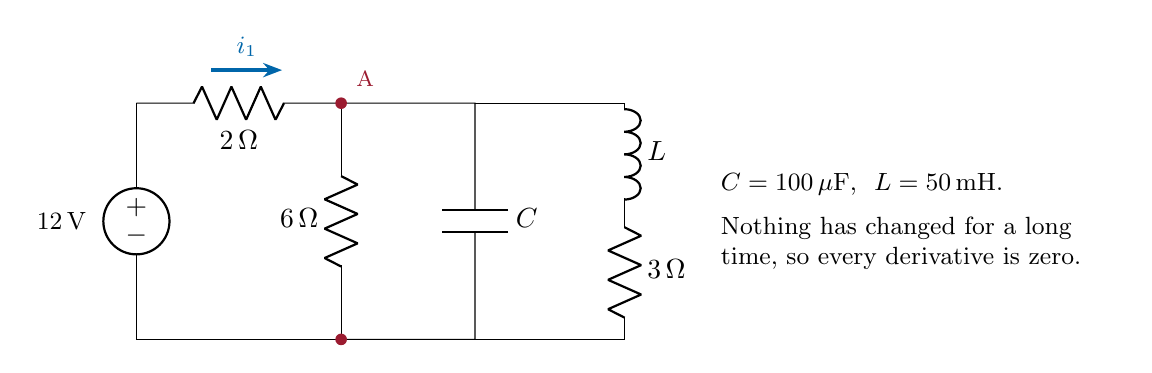
\begin{tikzpicture}[scale=1.0, transform shape]
  \draw (0,0) to[american voltage source, invert] (0,3.0);
  \node[font=\small] at (-0.95,1.5) {$12\V$};
  \draw (0,3.0) to[R, l_=$2\ohm$] (2.6,3.0);
  \draw[iar] (0.95,3.42) -- (1.85,3.42);
  \node[ccur, font=\small] at (1.4,3.72) {$i_1$};
  % middle branch: C parallel with 6 ohm
  \draw (2.6,3.0) to[R, l_=$6\ohm$] (2.6,0);
  \draw (2.6,3.0) -- (4.3,3.0) to[C, l=$C$] (4.3,0) -- (2.6,0);
  % right branch: L in series with 3 ohm
  \draw (4.3,3.0) -- (6.2,3.0) to[L, l=$L$] (6.2,1.7);
  \draw (6.2,1.7) to[R, l=$3\ohm$] (6.2,0);
  \draw (6.2,0) -- (0,0);
  \node[gnode] at (2.6,3.0) {};
  \node[gnode] at (2.6,0) {};
  \node[glab, above right=1pt and 2pt] at (2.6,3.05) {A};
  \node[font=\small, anchor=west, text width=5.0cm] at (7.3,1.5)
    {$C = 100\uni{\mu F}$, \ $L = 50\uni{mH}$.\\[5pt]
     Nothing has changed for a long time, so every derivative is zero.};
\end{tikzpicture}
\end{center}

\begin{examplebox}[Example 5.3 --- (a) find every branch variable in the steady state]


\textbf{Step 1 --- replace the two stores.} Nothing is changing, so by the table the
capacitor is an open circuit and the inductor a short circuit. What is left is Lecture~2's
resistive circuit.

\textbf{Step 2 --- solve it.} The $6\ohm$ and $3\ohm$ branches both run from node~A to the
bottom node, so
\[
  \Icol{i_1} = \frac{12}{2 + (6\parallel 3)} = \frac{12}{2+2} = 3\A ,
  \qquad
  \Vcol{v_A} = 12 - 2(3) = 6\V .
\]
\vspace{-12pt}
\[
  \Icol{i_{6\Omega}} = \frac{6}{6} = 1\A, \quad
  \Icol{i_{L}} = \Icol{i_{3\Omega}} = \frac{6}{3} = 2\A, \quad
  \Vcol{v_C} = 6\V, \quad \Vcol{v_L} = 0 , \quad \Icol{i_C} = 0 ,
\]
\vspace{-12pt}
\[
  \Pcol{w_C} = \tfrac12 (10^{-4})(6)^2 = 1.8\uni{mJ}, \qquad
  \Pcol{w_L} = \tfrac12 (0.05)(2)^2 = 0.1\J .
\]
\end{examplebox}

\begin{examplebox}[Example 5.3 --- (b) where is the power going?]
\[
  \Pcol{p_{\text{source}}} = -12 \times 3 = -36\W \ \text{(delivered)}, \qquad
  \Pcol{p_{2\Omega}} = 2(3)^2 = 18\W ,
\]
\vspace{-14pt}
\[
  \Pcol{p_{6\Omega}} = \frac{6^2}{6} = 6\W , \qquad
  \Pcol{p_{3\Omega}} = 3(2)^2 = 12\W .
\]
The resistors dissipate $18 + 6 + 12 = 36\W$, exactly what the source delivers. And the
two stores? The capacitor carries no current, the inductor has no voltage across it, so
\[
  \Pcol{p_C} = \Vcol{v_C}\,\Icol{i_C} = 6 \times 0 = 0 , \qquad
  \Pcol{p_L} = \Vcol{v_L}\,\Icol{i_L} = 0 \times 2 = 0 .
\]
\begin{center}
\emph{They hold energy. They do not consume any.}
\end{center}
The $1.8\uni{mJ}$ and the $0.1\J$ just sit there. Change something and they speak --- which
is what the next few lectures are about.
\end{examplebox}

%==============================================================
\section*{Summary}
\addcontentsline{toc}{section}{Summary}

\begin{itemize}
  \item An \textbf{inductor} fights changes in current, with a \textbf{back EMF}
        $\Vcol{v} = L\,d\Icol{i}/dt$. $L$ is in \textbf{henries}, set by the turn count,
        the winding's shape and what is inside it; one henry is large.
  \item Integrate the voltage: $\Fcol{\varphi} = \int\!\Vcol{v}\,d\tau$ in
        \textbf{volt-seconds} (webers), exactly as integrating the current gave charge in
        amp-seconds. An inductor is a curve in the $\Icol{i}$--$\Fcol{\varphi}$ plane; the
        \textbf{LTI} one is $\Fcol{\varphi} = L\Icol{i}$. Not a resistor --- no $f$ with
        $\Vcol{v(t)} = f(\Icol{i(t)})$.
  \item Short circuit at DC; its \textbf{current is continuous}; it remembers.
  \item Starting the current means \textbf{work against the back EMF}, and the total
        $\Pcol{w} = \tfrac12 L\Icol{i}^{\,2}$ is kept in the magnetic field and handed
        back in full: passive and \emph{lossless}. Forcing the current to jump demands a
        voltage impulse --- in a real switch, a spark.
  \item In a \textbf{DC steady state} the capacitor is open and the inductor short, so the
        circuit collapses to a resistive one and neither store absorbs power. Swap
        $\Vcol{v}\leftrightarrow\Icol{i}$, $\Qcol{q}\leftrightarrow\Fcol{\varphi}$,
        $C\leftrightarrow L$: the two stores are one element told twice
        (Section~\ref{sec:table}).
\end{itemize}

\subsection*{Next lecture}
\textbf{Dependent} sources --- whose value is set by a voltage or current elsewhere in the
circuit. They are how a transistor or an op-amp gets into a circuit diagram.

\subsection*{Reading}
\begin{itemize}
  \item Alexander \& Sadiku, \emph{Fundamentals of Electric Circuits}, Chapter~6.
  \item Chua, Desoer \& Kuh, \emph{Linear and Nonlinear Circuits}, Chapter~2.
  \item Lecture notes and videos of Prof.\ Emre Tuna,
        \href{https://users.metu.edu.tr/etuna/ee201/}{\texttt{users.metu.edu.tr/etuna/ee201}}
        --- Lecture~5: inductor $0{:}16$, LTI $4{:}51$, inductance $5{:}38$, power
        $9{:}49$, summary $12{:}35$, example $22{:}25$ and $33{:}01$.
\end{itemize}

\end{document}
